% ===================================================================
%                   Presentación con Latex Beamer
% ===================================================================
\documentclass[12pt,xcolor=svgnames]{beamer}
%\documentclass[handout,xcolor=svgnames]{beamer} %Version imprimible
% -------------------------------------------------------------------
% Paquetes personalizados
\usepackage{paquetes}
\usepackage{colores}
\usepackage{modo}
\usepackage{licencia}
\usepackage{eurosym}
\usepackage{graphics,epsfig, subfigure}
\usepackage{minted}
\setbeamertemplate{navigation symbols}{} 
\setbeamertemplate{footline}[frame number]

% -------------------------------------------------------------------
% Info
% ====
\title[Doxygen]{Documentación automática\\ con Doxygen}
\author[Noelia Sales]{Noelia Sales Montes\\\texttt{noelia.sales@uca.es}}
\institute[DV - UCA]{Diseño de Videojuegos\\
Universidad de Cádiz}
\date{}
% -------------------------------------------------------------------
\logo{
\includegraphics[width=1.5cm]{./img/logo}}

% Comienza el documento
\begin{document}
% Tikz -> Imágenes
\tikzstyle{every picture}+=[remember picture]
% Entorno matemático
\everymath{\displaystyle}
% -------------------------------------------------------------------

\begin{frame}
 \titlepage
\end{frame}

\begin{frame}{Repositorio}
  \url{http://github.com/nessa/taller-doxygen}
\end{frame}

\begin{frame}
\frametitle{Índice} 
\transboxin
\tableofcontents
\end{frame}

\section{Introducción}

\begin{frame}{Doxygen}
  \begin{center}
   {\large Doxygen es una herramienta de generación automática de
     documentación.}
 \end{center}

 \pause
 Permite:
 \begin{enumerate}
 \item<2-> Generar documentación on-line y manuales de referencia off-line.
 \item<3-> Extraer la estructura de ficheros de código \textbf{no
     documentados}.
 \item<4-> Generar documentación de ficheros \textbf{expresamente documentados}
   al ``estilo Doxygen''.
 \end{enumerate}
\end{frame}

\begin{frame}{¿Quién usa Doxygen?}
  \begin{itemize}
  \item Asterisk
  \item Gaim
  \item GNU (Standard C++ Library)
  \item GraphViz
  \item OGRE
  \item Pingus
  \item ScummVM
  \item Synergy
  \item ...\footnote{{\scriptsize \url{http://www.stack.nl/~dimitri/doxygen/projects.html}}}
  \end{itemize}
\end{frame}

\section{Funcionamiento}

\begin{frame}[fragile]{Instalación}
  GNU/Linux\footnote{Está disponible para la mayoría de distribuciones \\
    de GNU/Linux y para otros sistemas operativos.} - Distribuciones tipo
  Debian:
  \begin{minted}[fontsize=\footnotesize]{bash}
$ aptitude install doxygen texlive graphviz
$ aptitude install doxygen-gui doxymacs
  \end{minted}    
  \begin{itemize}
  \item \texttt{doxygen} $\longrightarrow$ Paquete completo
  \item \texttt{texlive} $\longrightarrow$ $\LaTeX$
  \item \texttt{graphviz} $\longrightarrow$ Generación de grafos
  \item \texttt{doxygen-gui} $\longrightarrow$ Interfaz gráfica (opcional)
  \item \texttt{doxymacs} $\longrightarrow$ Modo para Emacs
  \end{itemize}
\end{frame}

\begin{frame}{¿Cómo funciona Doxygen?}    
  \begin{cambiarmargen}{-1.2cm}{-1cm}
    \begin{figure}
      \centering
      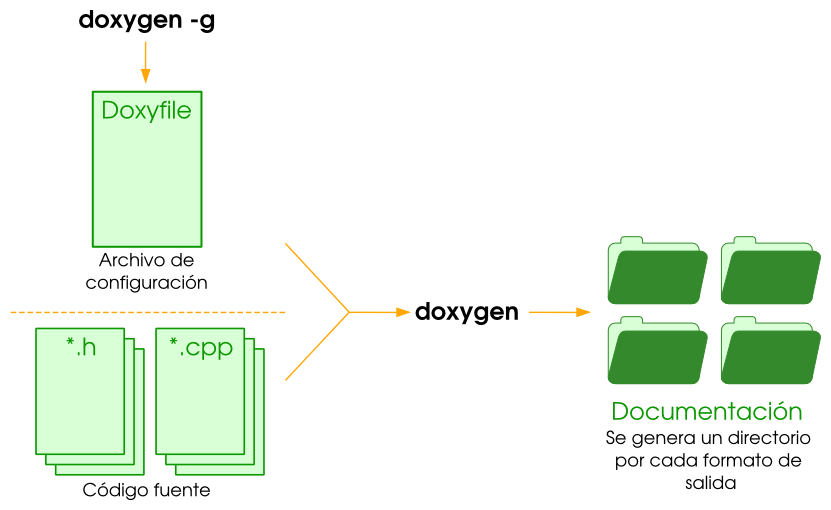
\includegraphics[width=1.1\textwidth]{./img/funcionamiento}
    \end{figure}
  \end{cambiarmargen}
\end{frame}

\begin{frame}{¿Cómo funciona Doxygen?}
  \begin{enumerate}
  \item Documentar el código.
  \item Generar el fichero de configuración: 
    \begin{center}\texttt{doxygen -g}\end{center}
  \item Editar el fichero de configuración.
  \item Generar la configuración:
    \begin{center}\texttt{doxygen [doxyfile]}\end{center}
  \end{enumerate}

  \begin{block}{}
    Si tienes un \textit{doxyfile} generado con una versión anterior de
    Doxygen, puedes actualizarlo:
    \begin{center}\texttt{doxygen -u [doxyfile]}\end{center}
  \end{block}
\end{frame}

\begin{frame}[fragile]{Doxyfile\footnote{{\scriptsize \url{http://www.stack.nl/~dimitri/doxygen/config.html}}}}
  Conjunto de:
  \begin{itemize}
  \item  \texttt{ETIQUETA = VALOR}
  \item \texttt{\# Comentarios}
  \end{itemize}
  \vspace*{0.5cm}
  Ejemplo:
{\scriptsize
\begin{verbatim}
DOXYFILE_ENCODING      = UTF-8

# The PROJECT_NAME tag is a single word (or a sequence of
# words surrounded by quotes) that should identify the project.

PROJECT_NAME           =                                      

# The PROJECT_NUMBER tag can be used to enter a project or revision
# number. This could be handy for archiving the generated
# documentation or if some version control system is used.                     

PROJECT_NUMBER         =  
\end{verbatim}
}
\end{frame}

\begin{frame}{Doxyfile}
  \begin{itemize}
  \item \texttt{PROJECT\_NAME = Proyecto}
  \item \texttt{INPUT = <fichero\_o\_directorio\_a\_leer>}
  \item \texttt{FILE\_PATTERNS = *.h, *.cpp}
  \item \texttt{OUTPUT\_LANGUAGE = English}
  \item \texttt{HAVE\_DOT = YES}
    \begin{itemize}
    \item  Usar GraphViz
    \end{itemize}
  \item \texttt{EXTRACT\_ALL = YES }
    \begin{itemize}
    \item Doxygen asumirá que todas las entidades están documentadas, aunque no
      sea así.
    \end{itemize}
  \end{itemize}
\end{frame}

\begin{frame}{Lenguajes de entrada}
  \begin{itemize}
  \item Lenguajes similares a C:
    \begin{itemize}
    \item C
    \item C++
    \item C\#
    \item Objective-C
    \item PHP
    \item Java
    \end{itemize}
  \item Python
  \item Fortran
  \item VHDL
  \item ...
  \end{itemize}
\end{frame}

\begin{frame}{Formatos de salida}
  \begin{block}{Directamente soportados}
    \begin{description}
    \item[HTML] \texttt{GENERATE\_HTML = YES}
    \item[$\LaTeX$] \texttt{GENERATE\_LATEX = YES}
    \item[Unix Man] \texttt{GENERATE\_MAN = YES}
    \item[XML] \texttt{GENERATE\_XML = YES}
    \end{description}
  \end{block}
  \begin{block}{Indirectamente soportados}
    \begin{description}
    \item[PDF]
      \begin{itemize}
      \item \texttt{ENABLE\_PDFLATEX = YES}
      \item \texttt{PDF\_HYPERLINKS = YES}
      \end{itemize}
    \end{description}
  \end{block}
\end{frame}

\begin{frame}[fragile]{Ejemplo 1}
  \begin{enumerate}
  \item Descargar \textit{octave} y crear el \textit{doxyfile}:\\
    {\scriptsize
\begin{verbatim}
mkdir ejemplo1 && cd ejemplo1
wget ftp://ftp.octave.org/gnu/octave/octave-3.6.1.tar.bz2
tar xjf octave-3.6.1
doxygen -g
\end{verbatim}
    }
  \item Editar el doxyfile:
    {\scriptsize
\begin{verbatim}
INPUT = octave-3.6.1/liboctave
FILE_PATTERNS = *.h
GENERATE_HTML = YES
GENERATE_LATEX = NO
EXTRACT_ALL = YES
\end{verbatim}
    }
  \item Ejecutar \texttt{doxygen}
  \item Ver \textit{html/index.html}
  \end{enumerate}
\end{frame}

\begin{frame}{Observaciones del ejemplo 1}
  \begin{itemize}
  \item Se generan enlaces de forma automática:
    \begin{itemize}
    \item Listado de ficheros
    \item Listados de clases (alfabético/jeraquizado) y de miembros
    \item En cada clase: 
      \begin{itemize}
      \item Enlace al fichero fuente
      \item Enlace a la documentación de cada miembro
      \end{itemize}
    \end{itemize}
  \item Se generan automáticamente diagramas de herencia
    \begin{itemize}
    \item \texttt{CLASS\_DIAGRAMS = YES}
    \end{itemize}
  \item Se pueden generar gráficos avanzados (GraphViz + \texttt{HAVE\_DOT =
      YES}):
    \begin{itemize}
    \item \texttt{GRAPHICAL\_HIERARCHY} (por defecto)
    \item \texttt{rCOLLABORATION\_GRAPH} (por defecto)
    \item \texttt{CALL\_GRAP}, \texttt{CALLER\_GRAPH}
    \end{itemize}
  \end{itemize}
\end{frame}

\section{Documentación}

\begin{frame}[fragile]{Bloques de documentación}
  \inputminted[fontsize=\footnotesize]{c++}{../materiales/codigo/coment.cpp}
\end{frame}

\begin{frame}{Documentación de un elemento\footnote{Todas son opcionales.}}
  \begin{enumerate}
  \item \textsc{Descripción corta}
    \begin{itemize}
    \item Explicación breve en una línea.
    \item Se puede indicar explícitamente con el parámetro \texttt{@brief}.
    \end{itemize}
  \item \textsc{Descripción larga}
    \begin{itemize}
    \item Párrafo con varias líneas.
    \item Es \textbf{necesario} indicar un salto de línea entre la descripción
      corta y ésta.
    \item \texttt{JAVADOC\_AUTOBRIEF = YES}: la descripción larga comienza tras
      el primer punto en comentarios tipo JavaDoc.
    \end{itemize}
  \item \textsc{Elementos adicionales}
  \end{enumerate}
\end{frame}

\begin{frame}{Elementos adicionales}
  \begin{itemize}
  \item \texttt{@author}
  \item \texttt{@date}
  \item \texttt{@exception}
  \item \texttt{@todo}
  \item \texttt{@\{ - @\}}: Agrupación de elementos.
  \item Otros: \texttt{@class}, \texttt{@union}, \texttt{@enum}, \texttt{@fn}
    (función), \texttt{@file}, \texttt{@typedef}, \texttt{@namespace},
    \texttt{@package}, \texttt{@interface}, ...
  \end{itemize}
\end{frame}

\begin{frame}[fragile]{Elementos adicionales}
  \inputminted[fontsize=\footnotesize,linenos=true]{c++}{../materiales/codigo/elem-adicionales.cpp}
\end{frame}

\begin{frame}{Ejemplo 2}
  \begin{enumerate}
  \item Entra en el subdirectorio \texttt{materiales/ejemplo2} del repositorio
  \item Genera el doxyfile: \texttt{doxygen -g}
    \begin{itemize}
    \item \texttt{HAVE\_DOT = NO}
    \item \texttt{HAVE\_DOT = YES}
    \end{itemize}
  \item Genera la documentación: \texttt{doxygen}
  \item Visualiza \textit{html/index.html}
  \end{enumerate}

  \begin{block}{}
  También se puede probar con \texttt{HAVE\_DOT = YES} en el proyecto de
    Octave, pero... tarda un poco ;)
  \end{block}
\end{frame}

\begin{frame}{Ejemplo 2}
    \begin{figure}
      \centering
      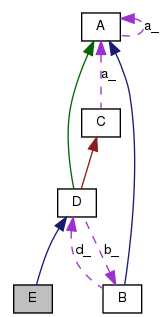
\includegraphics[scale=0.5]{./img/ejemplo2}
      \caption{Diagrama de colaboración de la clase E}
    \end{figure}
\end{frame}


\section{Conclusión}

\begin{frame}{Referencias y Agradecimientos}
  Referencias:
  \vspace*{0.2cm}
  {\scriptsize
  \begin{thebibliography}{6}
  \bibitem{} \url{http://www.stack.nl/~dimitri/doxygen/}
  \bibitem{} \url{http://www.stack.nl/~dimitri/doxygen/manual.html}
  \bibitem{} \url{http://trevinca.ei.uvigo.es/~jgarcia/FP/manuales/manualDoxygen.pdf}
  \end{thebibliography}
  }
  \vspace*{1cm}
  Agradecimientos a:
  \begin{itemize}
  \item Rafael Rodríguez Galván y José Tomás Tocino García, por poder
    inspirarme en sus talleres.
  \item Dimitri van Heesch, quien desarrolló y liberó Doxygen.
  \end{itemize}


\end{frame}

\begin{frame}{Para terminar}
  \begin{center}
    {\Large ¿Alguna pregunta?}
  \end{center}
\end{frame}

\licencia

\end{document}
